% Created by tikzDevice version 0.12.3.1 on 2022-08-15 11:15:43
% !TEX encoding = UTF-8 Unicode
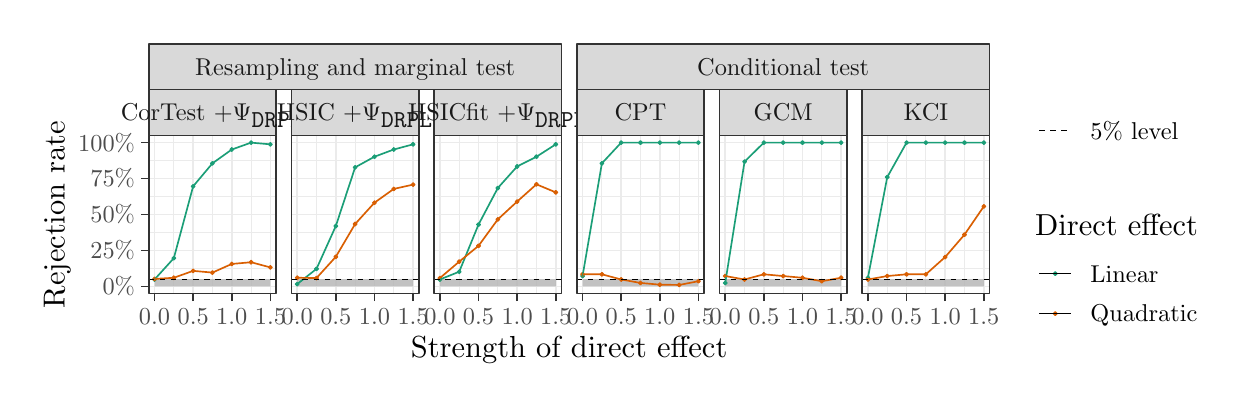
\begin{tikzpicture}[x=1pt,y=1pt]
\definecolor{fillColor}{RGB}{255,255,255}
\begin{scope}
\definecolor{drawColor}{RGB}{255,255,255}
\definecolor{fillColor}{RGB}{255,255,255}

\path[draw=drawColor,line width= 0.6pt,line join=round,line cap=round,fill=fillColor] (  0.00,  0.00) rectangle (433.62,126.47);
\end{scope}
\begin{scope}
\definecolor{fillColor}{RGB}{255,255,255}

\path[fill=fillColor] ( 43.44, 30.69) rectangle ( 89.50, 87.83);
\definecolor{drawColor}{gray}{0.92}

\path[draw=drawColor,line width= 0.3pt,line join=round] ( 43.44, 39.78) --
	( 89.50, 39.78);

\path[draw=drawColor,line width= 0.3pt,line join=round] ( 43.44, 52.76) --
	( 89.50, 52.76);

\path[draw=drawColor,line width= 0.3pt,line join=round] ( 43.44, 65.75) --
	( 89.50, 65.75);

\path[draw=drawColor,line width= 0.3pt,line join=round] ( 43.44, 78.74) --
	( 89.50, 78.74);

\path[draw=drawColor,line width= 0.3pt,line join=round] ( 52.51, 30.69) --
	( 52.51, 87.83);

\path[draw=drawColor,line width= 0.3pt,line join=round] ( 66.47, 30.69) --
	( 66.47, 87.83);

\path[draw=drawColor,line width= 0.3pt,line join=round] ( 80.43, 30.69) --
	( 80.43, 87.83);

\path[draw=drawColor,line width= 0.6pt,line join=round] ( 43.44, 33.28) --
	( 89.50, 33.28);

\path[draw=drawColor,line width= 0.6pt,line join=round] ( 43.44, 46.27) --
	( 89.50, 46.27);

\path[draw=drawColor,line width= 0.6pt,line join=round] ( 43.44, 59.26) --
	( 89.50, 59.26);

\path[draw=drawColor,line width= 0.6pt,line join=round] ( 43.44, 72.24) --
	( 89.50, 72.24);

\path[draw=drawColor,line width= 0.6pt,line join=round] ( 43.44, 85.23) --
	( 89.50, 85.23);

\path[draw=drawColor,line width= 0.6pt,line join=round] ( 45.54, 30.69) --
	( 45.54, 87.83);

\path[draw=drawColor,line width= 0.6pt,line join=round] ( 59.49, 30.69) --
	( 59.49, 87.83);

\path[draw=drawColor,line width= 0.6pt,line join=round] ( 73.45, 30.69) --
	( 73.45, 87.83);

\path[draw=drawColor,line width= 0.6pt,line join=round] ( 87.41, 30.69) --
	( 87.41, 87.83);
\definecolor{fillColor}{RGB}{179,179,179}

\path[fill=fillColor,fill opacity=0.80] ( 45.54, 35.88) --
	( 45.54, 35.88) --
	( 52.51, 35.88) --
	( 52.51, 35.88) --
	( 59.49, 35.88) --
	( 59.49, 35.88) --
	( 66.47, 35.88) --
	( 66.47, 35.88) --
	( 73.45, 35.88) --
	( 73.45, 35.88) --
	( 80.43, 35.88) --
	( 80.43, 35.88) --
	( 87.41, 35.88) --
	( 87.41, 35.88) --
	( 87.41, 33.28) --
	( 87.41, 33.28) --
	( 80.43, 33.28) --
	( 80.43, 33.28) --
	( 73.45, 33.28) --
	( 73.45, 33.28) --
	( 66.47, 33.28) --
	( 66.47, 33.28) --
	( 59.49, 33.28) --
	( 59.49, 33.28) --
	( 52.51, 33.28) --
	( 52.51, 33.28) --
	( 45.54, 33.28) --
	( 45.54, 33.28) --
	cycle;

\path[] ( 45.54, 35.88) --
	( 45.54, 35.88) --
	( 52.51, 35.88) --
	( 52.51, 35.88) --
	( 59.49, 35.88) --
	( 59.49, 35.88) --
	( 66.47, 35.88) --
	( 66.47, 35.88) --
	( 73.45, 35.88) --
	( 73.45, 35.88) --
	( 80.43, 35.88) --
	( 80.43, 35.88) --
	( 87.41, 35.88) --
	( 87.41, 35.88);

\path[] ( 87.41, 33.28) --
	( 87.41, 33.28) --
	( 80.43, 33.28) --
	( 80.43, 33.28) --
	( 73.45, 33.28) --
	( 73.45, 33.28) --
	( 66.47, 33.28) --
	( 66.47, 33.28) --
	( 59.49, 33.28) --
	( 59.49, 33.28) --
	( 52.51, 33.28) --
	( 52.51, 33.28) --
	( 45.54, 33.28) --
	( 45.54, 33.28);
\definecolor{drawColor}{RGB}{27,158,119}
\definecolor{fillColor}{RGB}{27,158,119}

\path[draw=drawColor,line width= 0.4pt,line join=round,line cap=round,fill=fillColor] ( 45.54, 35.78) circle (  0.68);
\definecolor{drawColor}{RGB}{217,95,2}
\definecolor{fillColor}{RGB}{217,95,2}

\path[draw=drawColor,line width= 0.4pt,line join=round,line cap=round,fill=fillColor] ( 45.54, 35.98) circle (  0.68);
\definecolor{drawColor}{RGB}{27,158,119}
\definecolor{fillColor}{RGB}{27,158,119}

\path[draw=drawColor,line width= 0.4pt,line join=round,line cap=round,fill=fillColor] ( 52.51, 43.47) circle (  0.68);
\definecolor{drawColor}{RGB}{217,95,2}
\definecolor{fillColor}{RGB}{217,95,2}

\path[draw=drawColor,line width= 0.4pt,line join=round,line cap=round,fill=fillColor] ( 52.51, 36.40) circle (  0.68);
\definecolor{drawColor}{RGB}{27,158,119}
\definecolor{fillColor}{RGB}{27,158,119}

\path[draw=drawColor,line width= 0.4pt,line join=round,line cap=round,fill=fillColor] ( 59.49, 69.44) circle (  0.68);
\definecolor{drawColor}{RGB}{217,95,2}
\definecolor{fillColor}{RGB}{217,95,2}

\path[draw=drawColor,line width= 0.4pt,line join=round,line cap=round,fill=fillColor] ( 59.49, 38.89) circle (  0.68);
\definecolor{drawColor}{RGB}{27,158,119}
\definecolor{fillColor}{RGB}{27,158,119}

\path[draw=drawColor,line width= 0.4pt,line join=round,line cap=round,fill=fillColor] ( 66.47, 77.75) circle (  0.68);
\definecolor{drawColor}{RGB}{217,95,2}
\definecolor{fillColor}{RGB}{217,95,2}

\path[draw=drawColor,line width= 0.4pt,line join=round,line cap=round,fill=fillColor] ( 66.47, 38.27) circle (  0.68);
\definecolor{drawColor}{RGB}{27,158,119}
\definecolor{fillColor}{RGB}{27,158,119}

\path[draw=drawColor,line width= 0.4pt,line join=round,line cap=round,fill=fillColor] ( 73.45, 82.74) circle (  0.68);
\definecolor{drawColor}{RGB}{217,95,2}
\definecolor{fillColor}{RGB}{217,95,2}

\path[draw=drawColor,line width= 0.4pt,line join=round,line cap=round,fill=fillColor] ( 73.45, 41.39) circle (  0.68);
\definecolor{drawColor}{RGB}{27,158,119}
\definecolor{fillColor}{RGB}{27,158,119}

\path[draw=drawColor,line width= 0.4pt,line join=round,line cap=round,fill=fillColor] ( 80.43, 85.23) circle (  0.68);
\definecolor{drawColor}{RGB}{217,95,2}
\definecolor{fillColor}{RGB}{217,95,2}

\path[draw=drawColor,line width= 0.4pt,line join=round,line cap=round,fill=fillColor] ( 80.43, 42.01) circle (  0.68);
\definecolor{drawColor}{RGB}{27,158,119}
\definecolor{fillColor}{RGB}{27,158,119}

\path[draw=drawColor,line width= 0.4pt,line join=round,line cap=round,fill=fillColor] ( 87.41, 84.61) circle (  0.68);
\definecolor{drawColor}{RGB}{217,95,2}
\definecolor{fillColor}{RGB}{217,95,2}

\path[draw=drawColor,line width= 0.4pt,line join=round,line cap=round,fill=fillColor] ( 87.41, 40.14) circle (  0.68);
\definecolor{drawColor}{RGB}{27,158,119}

\path[draw=drawColor,line width= 0.6pt,line join=round] ( 45.54, 35.78) --
	( 52.51, 43.47) --
	( 59.49, 69.44) --
	( 66.47, 77.75) --
	( 73.45, 82.74) --
	( 80.43, 85.23) --
	( 87.41, 84.61);
\definecolor{drawColor}{RGB}{217,95,2}

\path[draw=drawColor,line width= 0.6pt,line join=round] ( 45.54, 35.98) --
	( 52.51, 36.40) --
	( 59.49, 38.89) --
	( 66.47, 38.27) --
	( 73.45, 41.39) --
	( 80.43, 42.01) --
	( 87.41, 40.14);
\definecolor{drawColor}{RGB}{0,0,0}

\path[draw=drawColor,line width= 0.1pt,dash pattern=on 2pt off 2pt ,line join=round] ( 43.44, 35.88) -- ( 89.50, 35.88);
\definecolor{drawColor}{gray}{0.20}

\path[draw=drawColor,line width= 0.6pt,line join=round,line cap=round] ( 43.44, 30.69) rectangle ( 89.50, 87.83);
\end{scope}
\begin{scope}
\definecolor{fillColor}{RGB}{255,255,255}

\path[fill=fillColor] ( 95.00, 30.69) rectangle (141.06, 87.83);
\definecolor{drawColor}{gray}{0.92}

\path[draw=drawColor,line width= 0.3pt,line join=round] ( 95.00, 39.78) --
	(141.06, 39.78);

\path[draw=drawColor,line width= 0.3pt,line join=round] ( 95.00, 52.76) --
	(141.06, 52.76);

\path[draw=drawColor,line width= 0.3pt,line join=round] ( 95.00, 65.75) --
	(141.06, 65.75);

\path[draw=drawColor,line width= 0.3pt,line join=round] ( 95.00, 78.74) --
	(141.06, 78.74);

\path[draw=drawColor,line width= 0.3pt,line join=round] (104.07, 30.69) --
	(104.07, 87.83);

\path[draw=drawColor,line width= 0.3pt,line join=round] (118.03, 30.69) --
	(118.03, 87.83);

\path[draw=drawColor,line width= 0.3pt,line join=round] (131.98, 30.69) --
	(131.98, 87.83);

\path[draw=drawColor,line width= 0.6pt,line join=round] ( 95.00, 33.28) --
	(141.06, 33.28);

\path[draw=drawColor,line width= 0.6pt,line join=round] ( 95.00, 46.27) --
	(141.06, 46.27);

\path[draw=drawColor,line width= 0.6pt,line join=round] ( 95.00, 59.26) --
	(141.06, 59.26);

\path[draw=drawColor,line width= 0.6pt,line join=round] ( 95.00, 72.24) --
	(141.06, 72.24);

\path[draw=drawColor,line width= 0.6pt,line join=round] ( 95.00, 85.23) --
	(141.06, 85.23);

\path[draw=drawColor,line width= 0.6pt,line join=round] ( 97.09, 30.69) --
	( 97.09, 87.83);

\path[draw=drawColor,line width= 0.6pt,line join=round] (111.05, 30.69) --
	(111.05, 87.83);

\path[draw=drawColor,line width= 0.6pt,line join=round] (125.01, 30.69) --
	(125.01, 87.83);

\path[draw=drawColor,line width= 0.6pt,line join=round] (138.96, 30.69) --
	(138.96, 87.83);
\definecolor{fillColor}{RGB}{179,179,179}

\path[fill=fillColor,fill opacity=0.80] ( 97.09, 35.88) --
	( 97.09, 35.88) --
	(104.07, 35.88) --
	(104.07, 35.88) --
	(111.05, 35.88) --
	(111.05, 35.88) --
	(118.03, 35.88) --
	(118.03, 35.88) --
	(125.01, 35.88) --
	(125.01, 35.88) --
	(131.98, 35.88) --
	(131.98, 35.88) --
	(138.96, 35.88) --
	(138.96, 35.88) --
	(138.96, 33.28) --
	(138.96, 33.28) --
	(131.98, 33.28) --
	(131.98, 33.28) --
	(125.01, 33.28) --
	(125.01, 33.28) --
	(118.03, 33.28) --
	(118.03, 33.28) --
	(111.05, 33.28) --
	(111.05, 33.28) --
	(104.07, 33.28) --
	(104.07, 33.28) --
	( 97.09, 33.28) --
	( 97.09, 33.28) --
	cycle;

\path[] ( 97.09, 35.88) --
	( 97.09, 35.88) --
	(104.07, 35.88) --
	(104.07, 35.88) --
	(111.05, 35.88) --
	(111.05, 35.88) --
	(118.03, 35.88) --
	(118.03, 35.88) --
	(125.01, 35.88) --
	(125.01, 35.88) --
	(131.98, 35.88) --
	(131.98, 35.88) --
	(138.96, 35.88) --
	(138.96, 35.88);

\path[] (138.96, 33.28) --
	(138.96, 33.28) --
	(131.98, 33.28) --
	(131.98, 33.28) --
	(125.01, 33.28) --
	(125.01, 33.28) --
	(118.03, 33.28) --
	(118.03, 33.28) --
	(111.05, 33.28) --
	(111.05, 33.28) --
	(104.07, 33.28) --
	(104.07, 33.28) --
	( 97.09, 33.28) --
	( 97.09, 33.28);
\definecolor{drawColor}{RGB}{27,158,119}
\definecolor{fillColor}{RGB}{27,158,119}

\path[draw=drawColor,line width= 0.4pt,line join=round,line cap=round,fill=fillColor] ( 97.09, 34.11) circle (  0.68);
\definecolor{drawColor}{RGB}{217,95,2}
\definecolor{fillColor}{RGB}{217,95,2}

\path[draw=drawColor,line width= 0.4pt,line join=round,line cap=round,fill=fillColor] ( 97.09, 36.40) circle (  0.68);
\definecolor{drawColor}{RGB}{27,158,119}
\definecolor{fillColor}{RGB}{27,158,119}

\path[draw=drawColor,line width= 0.4pt,line join=round,line cap=round,fill=fillColor] (104.07, 39.62) circle (  0.68);
\definecolor{drawColor}{RGB}{217,95,2}
\definecolor{fillColor}{RGB}{217,95,2}

\path[draw=drawColor,line width= 0.4pt,line join=round,line cap=round,fill=fillColor] (104.07, 36.30) circle (  0.68);
\definecolor{drawColor}{RGB}{27,158,119}
\definecolor{fillColor}{RGB}{27,158,119}

\path[draw=drawColor,line width= 0.4pt,line join=round,line cap=round,fill=fillColor] (111.05, 55.10) circle (  0.68);
\definecolor{drawColor}{RGB}{217,95,2}
\definecolor{fillColor}{RGB}{217,95,2}

\path[draw=drawColor,line width= 0.4pt,line join=round,line cap=round,fill=fillColor] (111.05, 43.98) circle (  0.68);
\definecolor{drawColor}{RGB}{27,158,119}
\definecolor{fillColor}{RGB}{27,158,119}

\path[draw=drawColor,line width= 0.4pt,line join=round,line cap=round,fill=fillColor] (118.03, 76.30) circle (  0.68);
\definecolor{drawColor}{RGB}{217,95,2}
\definecolor{fillColor}{RGB}{217,95,2}

\path[draw=drawColor,line width= 0.4pt,line join=round,line cap=round,fill=fillColor] (118.03, 55.83) circle (  0.68);
\definecolor{drawColor}{RGB}{27,158,119}
\definecolor{fillColor}{RGB}{27,158,119}

\path[draw=drawColor,line width= 0.4pt,line join=round,line cap=round,fill=fillColor] (125.01, 80.14) circle (  0.68);
\definecolor{drawColor}{RGB}{217,95,2}
\definecolor{fillColor}{RGB}{217,95,2}

\path[draw=drawColor,line width= 0.4pt,line join=round,line cap=round,fill=fillColor] (125.01, 63.52) circle (  0.68);
\definecolor{drawColor}{RGB}{27,158,119}
\definecolor{fillColor}{RGB}{27,158,119}

\path[draw=drawColor,line width= 0.4pt,line join=round,line cap=round,fill=fillColor] (131.98, 82.74) circle (  0.68);
\definecolor{drawColor}{RGB}{217,95,2}
\definecolor{fillColor}{RGB}{217,95,2}

\path[draw=drawColor,line width= 0.4pt,line join=round,line cap=round,fill=fillColor] (131.98, 68.50) circle (  0.68);
\definecolor{drawColor}{RGB}{27,158,119}
\definecolor{fillColor}{RGB}{27,158,119}

\path[draw=drawColor,line width= 0.4pt,line join=round,line cap=round,fill=fillColor] (138.96, 84.61) circle (  0.68);
\definecolor{drawColor}{RGB}{217,95,2}
\definecolor{fillColor}{RGB}{217,95,2}

\path[draw=drawColor,line width= 0.4pt,line join=round,line cap=round,fill=fillColor] (138.96, 70.06) circle (  0.68);
\definecolor{drawColor}{RGB}{27,158,119}

\path[draw=drawColor,line width= 0.6pt,line join=round] ( 97.09, 34.11) --
	(104.07, 39.62) --
	(111.05, 55.10) --
	(118.03, 76.30) --
	(125.01, 80.14) --
	(131.98, 82.74) --
	(138.96, 84.61);
\definecolor{drawColor}{RGB}{217,95,2}

\path[draw=drawColor,line width= 0.6pt,line join=round] ( 97.09, 36.40) --
	(104.07, 36.30) --
	(111.05, 43.98) --
	(118.03, 55.83) --
	(125.01, 63.52) --
	(131.98, 68.50) --
	(138.96, 70.06);
\definecolor{drawColor}{RGB}{0,0,0}

\path[draw=drawColor,line width= 0.1pt,dash pattern=on 2pt off 2pt ,line join=round] ( 95.00, 35.88) -- (141.06, 35.88);
\definecolor{drawColor}{gray}{0.20}

\path[draw=drawColor,line width= 0.6pt,line join=round,line cap=round] ( 95.00, 30.69) rectangle (141.06, 87.83);
\end{scope}
\begin{scope}
\definecolor{fillColor}{RGB}{255,255,255}

\path[fill=fillColor] (146.56, 30.69) rectangle (192.61, 87.83);
\definecolor{drawColor}{gray}{0.92}

\path[draw=drawColor,line width= 0.3pt,line join=round] (146.56, 39.78) --
	(192.61, 39.78);

\path[draw=drawColor,line width= 0.3pt,line join=round] (146.56, 52.76) --
	(192.61, 52.76);

\path[draw=drawColor,line width= 0.3pt,line join=round] (146.56, 65.75) --
	(192.61, 65.75);

\path[draw=drawColor,line width= 0.3pt,line join=round] (146.56, 78.74) --
	(192.61, 78.74);

\path[draw=drawColor,line width= 0.3pt,line join=round] (155.63, 30.69) --
	(155.63, 87.83);

\path[draw=drawColor,line width= 0.3pt,line join=round] (169.58, 30.69) --
	(169.58, 87.83);

\path[draw=drawColor,line width= 0.3pt,line join=round] (183.54, 30.69) --
	(183.54, 87.83);

\path[draw=drawColor,line width= 0.6pt,line join=round] (146.56, 33.28) --
	(192.61, 33.28);

\path[draw=drawColor,line width= 0.6pt,line join=round] (146.56, 46.27) --
	(192.61, 46.27);

\path[draw=drawColor,line width= 0.6pt,line join=round] (146.56, 59.26) --
	(192.61, 59.26);

\path[draw=drawColor,line width= 0.6pt,line join=round] (146.56, 72.24) --
	(192.61, 72.24);

\path[draw=drawColor,line width= 0.6pt,line join=round] (146.56, 85.23) --
	(192.61, 85.23);

\path[draw=drawColor,line width= 0.6pt,line join=round] (148.65, 30.69) --
	(148.65, 87.83);

\path[draw=drawColor,line width= 0.6pt,line join=round] (162.61, 30.69) --
	(162.61, 87.83);

\path[draw=drawColor,line width= 0.6pt,line join=round] (176.56, 30.69) --
	(176.56, 87.83);

\path[draw=drawColor,line width= 0.6pt,line join=round] (190.52, 30.69) --
	(190.52, 87.83);
\definecolor{fillColor}{RGB}{179,179,179}

\path[fill=fillColor,fill opacity=0.80] (148.65, 35.88) --
	(148.65, 35.88) --
	(155.63, 35.88) --
	(155.63, 35.88) --
	(162.61, 35.88) --
	(162.61, 35.88) --
	(169.58, 35.88) --
	(169.58, 35.88) --
	(176.56, 35.88) --
	(176.56, 35.88) --
	(183.54, 35.88) --
	(183.54, 35.88) --
	(190.52, 35.88) --
	(190.52, 35.88) --
	(190.52, 33.28) --
	(190.52, 33.28) --
	(183.54, 33.28) --
	(183.54, 33.28) --
	(176.56, 33.28) --
	(176.56, 33.28) --
	(169.58, 33.28) --
	(169.58, 33.28) --
	(162.61, 33.28) --
	(162.61, 33.28) --
	(155.63, 33.28) --
	(155.63, 33.28) --
	(148.65, 33.28) --
	(148.65, 33.28) --
	cycle;

\path[] (148.65, 35.88) --
	(148.65, 35.88) --
	(155.63, 35.88) --
	(155.63, 35.88) --
	(162.61, 35.88) --
	(162.61, 35.88) --
	(169.58, 35.88) --
	(169.58, 35.88) --
	(176.56, 35.88) --
	(176.56, 35.88) --
	(183.54, 35.88) --
	(183.54, 35.88) --
	(190.52, 35.88) --
	(190.52, 35.88);

\path[] (190.52, 33.28) --
	(190.52, 33.28) --
	(183.54, 33.28) --
	(183.54, 33.28) --
	(176.56, 33.28) --
	(176.56, 33.28) --
	(169.58, 33.28) --
	(169.58, 33.28) --
	(162.61, 33.28) --
	(162.61, 33.28) --
	(155.63, 33.28) --
	(155.63, 33.28) --
	(148.65, 33.28) --
	(148.65, 33.28);
\definecolor{drawColor}{RGB}{27,158,119}
\definecolor{fillColor}{RGB}{27,158,119}

\path[draw=drawColor,line width= 0.4pt,line join=round,line cap=round,fill=fillColor] (148.65, 35.78) circle (  0.68);
\definecolor{drawColor}{RGB}{217,95,2}
\definecolor{fillColor}{RGB}{217,95,2}

\path[draw=drawColor,line width= 0.4pt,line join=round,line cap=round,fill=fillColor] (148.65, 36.30) circle (  0.68);
\definecolor{drawColor}{RGB}{27,158,119}
\definecolor{fillColor}{RGB}{27,158,119}

\path[draw=drawColor,line width= 0.4pt,line join=round,line cap=round,fill=fillColor] (155.63, 38.58) circle (  0.68);
\definecolor{drawColor}{RGB}{217,95,2}
\definecolor{fillColor}{RGB}{217,95,2}

\path[draw=drawColor,line width= 0.4pt,line join=round,line cap=round,fill=fillColor] (155.63, 42.22) circle (  0.68);
\definecolor{drawColor}{RGB}{27,158,119}
\definecolor{fillColor}{RGB}{27,158,119}

\path[draw=drawColor,line width= 0.4pt,line join=round,line cap=round,fill=fillColor] (162.61, 55.62) circle (  0.68);
\definecolor{drawColor}{RGB}{217,95,2}
\definecolor{fillColor}{RGB}{217,95,2}

\path[draw=drawColor,line width= 0.4pt,line join=round,line cap=round,fill=fillColor] (162.61, 47.93) circle (  0.68);
\definecolor{drawColor}{RGB}{27,158,119}
\definecolor{fillColor}{RGB}{27,158,119}

\path[draw=drawColor,line width= 0.4pt,line join=round,line cap=round,fill=fillColor] (169.58, 68.82) circle (  0.68);
\definecolor{drawColor}{RGB}{217,95,2}
\definecolor{fillColor}{RGB}{217,95,2}

\path[draw=drawColor,line width= 0.4pt,line join=round,line cap=round,fill=fillColor] (169.58, 57.49) circle (  0.68);
\definecolor{drawColor}{RGB}{27,158,119}
\definecolor{fillColor}{RGB}{27,158,119}

\path[draw=drawColor,line width= 0.4pt,line join=round,line cap=round,fill=fillColor] (176.56, 76.61) circle (  0.68);
\definecolor{drawColor}{RGB}{217,95,2}
\definecolor{fillColor}{RGB}{217,95,2}

\path[draw=drawColor,line width= 0.4pt,line join=round,line cap=round,fill=fillColor] (176.56, 63.93) circle (  0.68);
\definecolor{drawColor}{RGB}{27,158,119}
\definecolor{fillColor}{RGB}{27,158,119}

\path[draw=drawColor,line width= 0.4pt,line join=round,line cap=round,fill=fillColor] (183.54, 80.14) circle (  0.68);
\definecolor{drawColor}{RGB}{217,95,2}
\definecolor{fillColor}{RGB}{217,95,2}

\path[draw=drawColor,line width= 0.4pt,line join=round,line cap=round,fill=fillColor] (183.54, 70.17) circle (  0.68);
\definecolor{drawColor}{RGB}{27,158,119}
\definecolor{fillColor}{RGB}{27,158,119}

\path[draw=drawColor,line width= 0.4pt,line join=round,line cap=round,fill=fillColor] (190.52, 84.61) circle (  0.68);
\definecolor{drawColor}{RGB}{217,95,2}
\definecolor{fillColor}{RGB}{217,95,2}

\path[draw=drawColor,line width= 0.4pt,line join=round,line cap=round,fill=fillColor] (190.52, 67.26) circle (  0.68);
\definecolor{drawColor}{RGB}{27,158,119}

\path[draw=drawColor,line width= 0.6pt,line join=round] (148.65, 35.78) --
	(155.63, 38.58) --
	(162.61, 55.62) --
	(169.58, 68.82) --
	(176.56, 76.61) --
	(183.54, 80.14) --
	(190.52, 84.61);
\definecolor{drawColor}{RGB}{217,95,2}

\path[draw=drawColor,line width= 0.6pt,line join=round] (148.65, 36.30) --
	(155.63, 42.22) --
	(162.61, 47.93) --
	(169.58, 57.49) --
	(176.56, 63.93) --
	(183.54, 70.17) --
	(190.52, 67.26);
\definecolor{drawColor}{RGB}{0,0,0}

\path[draw=drawColor,line width= 0.1pt,dash pattern=on 2pt off 2pt ,line join=round] (146.56, 35.88) -- (192.61, 35.88);
\definecolor{drawColor}{gray}{0.20}

\path[draw=drawColor,line width= 0.6pt,line join=round,line cap=round] (146.56, 30.69) rectangle (192.61, 87.83);
\end{scope}
\begin{scope}
\definecolor{fillColor}{RGB}{255,255,255}

\path[fill=fillColor] (198.11, 30.69) rectangle (244.17, 87.83);
\definecolor{drawColor}{gray}{0.92}

\path[draw=drawColor,line width= 0.3pt,line join=round] (198.11, 39.78) --
	(244.17, 39.78);

\path[draw=drawColor,line width= 0.3pt,line join=round] (198.11, 52.76) --
	(244.17, 52.76);

\path[draw=drawColor,line width= 0.3pt,line join=round] (198.11, 65.75) --
	(244.17, 65.75);

\path[draw=drawColor,line width= 0.3pt,line join=round] (198.11, 78.74) --
	(244.17, 78.74);

\path[draw=drawColor,line width= 0.3pt,line join=round] (207.19, 30.69) --
	(207.19, 87.83);

\path[draw=drawColor,line width= 0.3pt,line join=round] (221.14, 30.69) --
	(221.14, 87.83);

\path[draw=drawColor,line width= 0.3pt,line join=round] (235.10, 30.69) --
	(235.10, 87.83);

\path[draw=drawColor,line width= 0.6pt,line join=round] (198.11, 33.28) --
	(244.17, 33.28);

\path[draw=drawColor,line width= 0.6pt,line join=round] (198.11, 46.27) --
	(244.17, 46.27);

\path[draw=drawColor,line width= 0.6pt,line join=round] (198.11, 59.26) --
	(244.17, 59.26);

\path[draw=drawColor,line width= 0.6pt,line join=round] (198.11, 72.24) --
	(244.17, 72.24);

\path[draw=drawColor,line width= 0.6pt,line join=round] (198.11, 85.23) --
	(244.17, 85.23);

\path[draw=drawColor,line width= 0.6pt,line join=round] (200.21, 30.69) --
	(200.21, 87.83);

\path[draw=drawColor,line width= 0.6pt,line join=round] (214.16, 30.69) --
	(214.16, 87.83);

\path[draw=drawColor,line width= 0.6pt,line join=round] (228.12, 30.69) --
	(228.12, 87.83);

\path[draw=drawColor,line width= 0.6pt,line join=round] (242.08, 30.69) --
	(242.08, 87.83);
\definecolor{fillColor}{RGB}{179,179,179}

\path[fill=fillColor,fill opacity=0.80] (200.21, 35.88) --
	(200.21, 35.88) --
	(207.19, 35.88) --
	(207.19, 35.88) --
	(214.16, 35.88) --
	(214.16, 35.88) --
	(221.14, 35.88) --
	(221.14, 35.88) --
	(228.12, 35.88) --
	(228.12, 35.88) --
	(235.10, 35.88) --
	(235.10, 35.88) --
	(242.08, 35.88) --
	(242.08, 35.88) --
	(242.08, 33.28) --
	(242.08, 33.28) --
	(235.10, 33.28) --
	(235.10, 33.28) --
	(228.12, 33.28) --
	(228.12, 33.28) --
	(221.14, 33.28) --
	(221.14, 33.28) --
	(214.16, 33.28) --
	(214.16, 33.28) --
	(207.19, 33.28) --
	(207.19, 33.28) --
	(200.21, 33.28) --
	(200.21, 33.28) --
	cycle;

\path[] (200.21, 35.88) --
	(200.21, 35.88) --
	(207.19, 35.88) --
	(207.19, 35.88) --
	(214.16, 35.88) --
	(214.16, 35.88) --
	(221.14, 35.88) --
	(221.14, 35.88) --
	(228.12, 35.88) --
	(228.12, 35.88) --
	(235.10, 35.88) --
	(235.10, 35.88) --
	(242.08, 35.88) --
	(242.08, 35.88);

\path[] (242.08, 33.28) --
	(242.08, 33.28) --
	(235.10, 33.28) --
	(235.10, 33.28) --
	(228.12, 33.28) --
	(228.12, 33.28) --
	(221.14, 33.28) --
	(221.14, 33.28) --
	(214.16, 33.28) --
	(214.16, 33.28) --
	(207.19, 33.28) --
	(207.19, 33.28) --
	(200.21, 33.28) --
	(200.21, 33.28);
\definecolor{drawColor}{RGB}{27,158,119}
\definecolor{fillColor}{RGB}{27,158,119}

\path[draw=drawColor,line width= 0.4pt,line join=round,line cap=round,fill=fillColor] (200.21, 37.02) circle (  0.68);
\definecolor{drawColor}{RGB}{217,95,2}
\definecolor{fillColor}{RGB}{217,95,2}

\path[draw=drawColor,line width= 0.4pt,line join=round,line cap=round,fill=fillColor] (200.21, 37.65) circle (  0.68);
\definecolor{drawColor}{RGB}{27,158,119}
\definecolor{fillColor}{RGB}{27,158,119}

\path[draw=drawColor,line width= 0.4pt,line join=round,line cap=round,fill=fillColor] (207.19, 77.75) circle (  0.68);
\definecolor{drawColor}{RGB}{217,95,2}
\definecolor{fillColor}{RGB}{217,95,2}

\path[draw=drawColor,line width= 0.4pt,line join=round,line cap=round,fill=fillColor] (207.19, 37.65) circle (  0.68);
\definecolor{drawColor}{RGB}{27,158,119}
\definecolor{fillColor}{RGB}{27,158,119}

\path[draw=drawColor,line width= 0.4pt,line join=round,line cap=round,fill=fillColor] (214.16, 85.23) circle (  0.68);
\definecolor{drawColor}{RGB}{217,95,2}
\definecolor{fillColor}{RGB}{217,95,2}

\path[draw=drawColor,line width= 0.4pt,line join=round,line cap=round,fill=fillColor] (214.16, 35.78) circle (  0.68);
\definecolor{drawColor}{RGB}{27,158,119}
\definecolor{fillColor}{RGB}{27,158,119}

\path[draw=drawColor,line width= 0.4pt,line join=round,line cap=round,fill=fillColor] (221.14, 85.23) circle (  0.68);
\definecolor{drawColor}{RGB}{217,95,2}
\definecolor{fillColor}{RGB}{217,95,2}

\path[draw=drawColor,line width= 0.4pt,line join=round,line cap=round,fill=fillColor] (221.14, 34.53) circle (  0.68);
\definecolor{drawColor}{RGB}{27,158,119}
\definecolor{fillColor}{RGB}{27,158,119}

\path[draw=drawColor,line width= 0.4pt,line join=round,line cap=round,fill=fillColor] (228.12, 85.23) circle (  0.68);
\definecolor{drawColor}{RGB}{217,95,2}
\definecolor{fillColor}{RGB}{217,95,2}

\path[draw=drawColor,line width= 0.4pt,line join=round,line cap=round,fill=fillColor] (228.12, 33.91) circle (  0.68);
\definecolor{drawColor}{RGB}{27,158,119}
\definecolor{fillColor}{RGB}{27,158,119}

\path[draw=drawColor,line width= 0.4pt,line join=round,line cap=round,fill=fillColor] (235.10, 85.23) circle (  0.68);
\definecolor{drawColor}{RGB}{217,95,2}
\definecolor{fillColor}{RGB}{217,95,2}

\path[draw=drawColor,line width= 0.4pt,line join=round,line cap=round,fill=fillColor] (235.10, 33.80) circle (  0.68);
\definecolor{drawColor}{RGB}{27,158,119}
\definecolor{fillColor}{RGB}{27,158,119}

\path[draw=drawColor,line width= 0.4pt,line join=round,line cap=round,fill=fillColor] (242.08, 85.23) circle (  0.68);
\definecolor{drawColor}{RGB}{217,95,2}
\definecolor{fillColor}{RGB}{217,95,2}

\path[draw=drawColor,line width= 0.4pt,line join=round,line cap=round,fill=fillColor] (242.08, 35.15) circle (  0.68);
\definecolor{drawColor}{RGB}{27,158,119}

\path[draw=drawColor,line width= 0.6pt,line join=round] (200.21, 37.02) --
	(207.19, 77.75) --
	(214.16, 85.23) --
	(221.14, 85.23) --
	(228.12, 85.23) --
	(235.10, 85.23) --
	(242.08, 85.23);
\definecolor{drawColor}{RGB}{217,95,2}

\path[draw=drawColor,line width= 0.6pt,line join=round] (200.21, 37.65) --
	(207.19, 37.65) --
	(214.16, 35.78) --
	(221.14, 34.53) --
	(228.12, 33.91) --
	(235.10, 33.80) --
	(242.08, 35.15);
\definecolor{drawColor}{RGB}{0,0,0}

\path[draw=drawColor,line width= 0.1pt,dash pattern=on 2pt off 2pt ,line join=round] (198.11, 35.88) -- (244.17, 35.88);
\definecolor{drawColor}{gray}{0.20}

\path[draw=drawColor,line width= 0.6pt,line join=round,line cap=round] (198.11, 30.69) rectangle (244.17, 87.83);
\end{scope}
\begin{scope}
\definecolor{fillColor}{RGB}{255,255,255}

\path[fill=fillColor] (249.67, 30.69) rectangle (295.73, 87.83);
\definecolor{drawColor}{gray}{0.92}

\path[draw=drawColor,line width= 0.3pt,line join=round] (249.67, 39.78) --
	(295.73, 39.78);

\path[draw=drawColor,line width= 0.3pt,line join=round] (249.67, 52.76) --
	(295.73, 52.76);

\path[draw=drawColor,line width= 0.3pt,line join=round] (249.67, 65.75) --
	(295.73, 65.75);

\path[draw=drawColor,line width= 0.3pt,line join=round] (249.67, 78.74) --
	(295.73, 78.74);

\path[draw=drawColor,line width= 0.3pt,line join=round] (258.74, 30.69) --
	(258.74, 87.83);

\path[draw=drawColor,line width= 0.3pt,line join=round] (272.70, 30.69) --
	(272.70, 87.83);

\path[draw=drawColor,line width= 0.3pt,line join=round] (286.66, 30.69) --
	(286.66, 87.83);

\path[draw=drawColor,line width= 0.6pt,line join=round] (249.67, 33.28) --
	(295.73, 33.28);

\path[draw=drawColor,line width= 0.6pt,line join=round] (249.67, 46.27) --
	(295.73, 46.27);

\path[draw=drawColor,line width= 0.6pt,line join=round] (249.67, 59.26) --
	(295.73, 59.26);

\path[draw=drawColor,line width= 0.6pt,line join=round] (249.67, 72.24) --
	(295.73, 72.24);

\path[draw=drawColor,line width= 0.6pt,line join=round] (249.67, 85.23) --
	(295.73, 85.23);

\path[draw=drawColor,line width= 0.6pt,line join=round] (251.76, 30.69) --
	(251.76, 87.83);

\path[draw=drawColor,line width= 0.6pt,line join=round] (265.72, 30.69) --
	(265.72, 87.83);

\path[draw=drawColor,line width= 0.6pt,line join=round] (279.68, 30.69) --
	(279.68, 87.83);

\path[draw=drawColor,line width= 0.6pt,line join=round] (293.63, 30.69) --
	(293.63, 87.83);
\definecolor{fillColor}{RGB}{179,179,179}

\path[fill=fillColor,fill opacity=0.80] (251.76, 35.88) --
	(251.76, 35.88) --
	(258.74, 35.88) --
	(258.74, 35.88) --
	(265.72, 35.88) --
	(265.72, 35.88) --
	(272.70, 35.88) --
	(272.70, 35.88) --
	(279.68, 35.88) --
	(279.68, 35.88) --
	(286.66, 35.88) --
	(286.66, 35.88) --
	(293.63, 35.88) --
	(293.63, 35.88) --
	(293.63, 33.28) --
	(293.63, 33.28) --
	(286.66, 33.28) --
	(286.66, 33.28) --
	(279.68, 33.28) --
	(279.68, 33.28) --
	(272.70, 33.28) --
	(272.70, 33.28) --
	(265.72, 33.28) --
	(265.72, 33.28) --
	(258.74, 33.28) --
	(258.74, 33.28) --
	(251.76, 33.28) --
	(251.76, 33.28) --
	cycle;

\path[] (251.76, 35.88) --
	(251.76, 35.88) --
	(258.74, 35.88) --
	(258.74, 35.88) --
	(265.72, 35.88) --
	(265.72, 35.88) --
	(272.70, 35.88) --
	(272.70, 35.88) --
	(279.68, 35.88) --
	(279.68, 35.88) --
	(286.66, 35.88) --
	(286.66, 35.88) --
	(293.63, 35.88) --
	(293.63, 35.88);

\path[] (293.63, 33.28) --
	(293.63, 33.28) --
	(286.66, 33.28) --
	(286.66, 33.28) --
	(279.68, 33.28) --
	(279.68, 33.28) --
	(272.70, 33.28) --
	(272.70, 33.28) --
	(265.72, 33.28) --
	(265.72, 33.28) --
	(258.74, 33.28) --
	(258.74, 33.28) --
	(251.76, 33.28) --
	(251.76, 33.28);
\definecolor{drawColor}{RGB}{27,158,119}
\definecolor{fillColor}{RGB}{27,158,119}

\path[draw=drawColor,line width= 0.4pt,line join=round,line cap=round,fill=fillColor] (251.76, 34.53) circle (  0.68);
\definecolor{drawColor}{RGB}{217,95,2}
\definecolor{fillColor}{RGB}{217,95,2}

\path[draw=drawColor,line width= 0.4pt,line join=round,line cap=round,fill=fillColor] (251.76, 37.02) circle (  0.68);
\definecolor{drawColor}{RGB}{27,158,119}
\definecolor{fillColor}{RGB}{27,158,119}

\path[draw=drawColor,line width= 0.4pt,line join=round,line cap=round,fill=fillColor] (258.74, 78.37) circle (  0.68);
\definecolor{drawColor}{RGB}{217,95,2}
\definecolor{fillColor}{RGB}{217,95,2}

\path[draw=drawColor,line width= 0.4pt,line join=round,line cap=round,fill=fillColor] (258.74, 35.78) circle (  0.68);
\definecolor{drawColor}{RGB}{27,158,119}
\definecolor{fillColor}{RGB}{27,158,119}

\path[draw=drawColor,line width= 0.4pt,line join=round,line cap=round,fill=fillColor] (265.72, 85.23) circle (  0.68);
\definecolor{drawColor}{RGB}{217,95,2}
\definecolor{fillColor}{RGB}{217,95,2}

\path[draw=drawColor,line width= 0.4pt,line join=round,line cap=round,fill=fillColor] (265.72, 37.65) circle (  0.68);
\definecolor{drawColor}{RGB}{27,158,119}
\definecolor{fillColor}{RGB}{27,158,119}

\path[draw=drawColor,line width= 0.4pt,line join=round,line cap=round,fill=fillColor] (272.70, 85.23) circle (  0.68);
\definecolor{drawColor}{RGB}{217,95,2}
\definecolor{fillColor}{RGB}{217,95,2}

\path[draw=drawColor,line width= 0.4pt,line join=round,line cap=round,fill=fillColor] (272.70, 37.02) circle (  0.68);
\definecolor{drawColor}{RGB}{27,158,119}
\definecolor{fillColor}{RGB}{27,158,119}

\path[draw=drawColor,line width= 0.4pt,line join=round,line cap=round,fill=fillColor] (279.68, 85.23) circle (  0.68);
\definecolor{drawColor}{RGB}{217,95,2}
\definecolor{fillColor}{RGB}{217,95,2}

\path[draw=drawColor,line width= 0.4pt,line join=round,line cap=round,fill=fillColor] (279.68, 36.40) circle (  0.68);
\definecolor{drawColor}{RGB}{27,158,119}
\definecolor{fillColor}{RGB}{27,158,119}

\path[draw=drawColor,line width= 0.4pt,line join=round,line cap=round,fill=fillColor] (286.66, 85.23) circle (  0.68);
\definecolor{drawColor}{RGB}{217,95,2}
\definecolor{fillColor}{RGB}{217,95,2}

\path[draw=drawColor,line width= 0.4pt,line join=round,line cap=round,fill=fillColor] (286.66, 35.15) circle (  0.68);
\definecolor{drawColor}{RGB}{27,158,119}
\definecolor{fillColor}{RGB}{27,158,119}

\path[draw=drawColor,line width= 0.4pt,line join=round,line cap=round,fill=fillColor] (293.63, 85.23) circle (  0.68);
\definecolor{drawColor}{RGB}{217,95,2}
\definecolor{fillColor}{RGB}{217,95,2}

\path[draw=drawColor,line width= 0.4pt,line join=round,line cap=round,fill=fillColor] (293.63, 36.40) circle (  0.68);
\definecolor{drawColor}{RGB}{27,158,119}

\path[draw=drawColor,line width= 0.6pt,line join=round] (251.76, 34.53) --
	(258.74, 78.37) --
	(265.72, 85.23) --
	(272.70, 85.23) --
	(279.68, 85.23) --
	(286.66, 85.23) --
	(293.63, 85.23);
\definecolor{drawColor}{RGB}{217,95,2}

\path[draw=drawColor,line width= 0.6pt,line join=round] (251.76, 37.02) --
	(258.74, 35.78) --
	(265.72, 37.65) --
	(272.70, 37.02) --
	(279.68, 36.40) --
	(286.66, 35.15) --
	(293.63, 36.40);
\definecolor{drawColor}{RGB}{0,0,0}

\path[draw=drawColor,line width= 0.1pt,dash pattern=on 2pt off 2pt ,line join=round] (249.67, 35.88) -- (295.73, 35.88);
\definecolor{drawColor}{gray}{0.20}

\path[draw=drawColor,line width= 0.6pt,line join=round,line cap=round] (249.67, 30.69) rectangle (295.73, 87.83);
\end{scope}
\begin{scope}
\definecolor{fillColor}{RGB}{255,255,255}

\path[fill=fillColor] (301.23, 30.69) rectangle (347.28, 87.83);
\definecolor{drawColor}{gray}{0.92}

\path[draw=drawColor,line width= 0.3pt,line join=round] (301.23, 39.78) --
	(347.28, 39.78);

\path[draw=drawColor,line width= 0.3pt,line join=round] (301.23, 52.76) --
	(347.28, 52.76);

\path[draw=drawColor,line width= 0.3pt,line join=round] (301.23, 65.75) --
	(347.28, 65.75);

\path[draw=drawColor,line width= 0.3pt,line join=round] (301.23, 78.74) --
	(347.28, 78.74);

\path[draw=drawColor,line width= 0.3pt,line join=round] (310.30, 30.69) --
	(310.30, 87.83);

\path[draw=drawColor,line width= 0.3pt,line join=round] (324.26, 30.69) --
	(324.26, 87.83);

\path[draw=drawColor,line width= 0.3pt,line join=round] (338.21, 30.69) --
	(338.21, 87.83);

\path[draw=drawColor,line width= 0.6pt,line join=round] (301.23, 33.28) --
	(347.28, 33.28);

\path[draw=drawColor,line width= 0.6pt,line join=round] (301.23, 46.27) --
	(347.28, 46.27);

\path[draw=drawColor,line width= 0.6pt,line join=round] (301.23, 59.26) --
	(347.28, 59.26);

\path[draw=drawColor,line width= 0.6pt,line join=round] (301.23, 72.24) --
	(347.28, 72.24);

\path[draw=drawColor,line width= 0.6pt,line join=round] (301.23, 85.23) --
	(347.28, 85.23);

\path[draw=drawColor,line width= 0.6pt,line join=round] (303.32, 30.69) --
	(303.32, 87.83);

\path[draw=drawColor,line width= 0.6pt,line join=round] (317.28, 30.69) --
	(317.28, 87.83);

\path[draw=drawColor,line width= 0.6pt,line join=round] (331.23, 30.69) --
	(331.23, 87.83);

\path[draw=drawColor,line width= 0.6pt,line join=round] (345.19, 30.69) --
	(345.19, 87.83);
\definecolor{fillColor}{RGB}{179,179,179}

\path[fill=fillColor,fill opacity=0.80] (303.32, 35.88) --
	(303.32, 35.88) --
	(310.30, 35.88) --
	(310.30, 35.88) --
	(317.28, 35.88) --
	(317.28, 35.88) --
	(324.26, 35.88) --
	(324.26, 35.88) --
	(331.23, 35.88) --
	(331.23, 35.88) --
	(338.21, 35.88) --
	(338.21, 35.88) --
	(345.19, 35.88) --
	(345.19, 35.88) --
	(345.19, 33.28) --
	(345.19, 33.28) --
	(338.21, 33.28) --
	(338.21, 33.28) --
	(331.23, 33.28) --
	(331.23, 33.28) --
	(324.26, 33.28) --
	(324.26, 33.28) --
	(317.28, 33.28) --
	(317.28, 33.28) --
	(310.30, 33.28) --
	(310.30, 33.28) --
	(303.32, 33.28) --
	(303.32, 33.28) --
	cycle;

\path[] (303.32, 35.88) --
	(303.32, 35.88) --
	(310.30, 35.88) --
	(310.30, 35.88) --
	(317.28, 35.88) --
	(317.28, 35.88) --
	(324.26, 35.88) --
	(324.26, 35.88) --
	(331.23, 35.88) --
	(331.23, 35.88) --
	(338.21, 35.88) --
	(338.21, 35.88) --
	(345.19, 35.88) --
	(345.19, 35.88);

\path[] (345.19, 33.28) --
	(345.19, 33.28) --
	(338.21, 33.28) --
	(338.21, 33.28) --
	(331.23, 33.28) --
	(331.23, 33.28) --
	(324.26, 33.28) --
	(324.26, 33.28) --
	(317.28, 33.28) --
	(317.28, 33.28) --
	(310.30, 33.28) --
	(310.30, 33.28) --
	(303.32, 33.28) --
	(303.32, 33.28);
\definecolor{drawColor}{RGB}{27,158,119}
\definecolor{fillColor}{RGB}{27,158,119}

\path[draw=drawColor,line width= 0.4pt,line join=round,line cap=round,fill=fillColor] (303.32, 36.40) circle (  0.68);
\definecolor{drawColor}{RGB}{217,95,2}
\definecolor{fillColor}{RGB}{217,95,2}

\path[draw=drawColor,line width= 0.4pt,line join=round,line cap=round,fill=fillColor] (303.32, 35.78) circle (  0.68);
\definecolor{drawColor}{RGB}{27,158,119}
\definecolor{fillColor}{RGB}{27,158,119}

\path[draw=drawColor,line width= 0.4pt,line join=round,line cap=round,fill=fillColor] (310.30, 72.76) circle (  0.68);
\definecolor{drawColor}{RGB}{217,95,2}
\definecolor{fillColor}{RGB}{217,95,2}

\path[draw=drawColor,line width= 0.4pt,line join=round,line cap=round,fill=fillColor] (310.30, 37.02) circle (  0.68);
\definecolor{drawColor}{RGB}{27,158,119}
\definecolor{fillColor}{RGB}{27,158,119}

\path[draw=drawColor,line width= 0.4pt,line join=round,line cap=round,fill=fillColor] (317.28, 85.23) circle (  0.68);
\definecolor{drawColor}{RGB}{217,95,2}
\definecolor{fillColor}{RGB}{217,95,2}

\path[draw=drawColor,line width= 0.4pt,line join=round,line cap=round,fill=fillColor] (317.28, 37.65) circle (  0.68);
\definecolor{drawColor}{RGB}{27,158,119}
\definecolor{fillColor}{RGB}{27,158,119}

\path[draw=drawColor,line width= 0.4pt,line join=round,line cap=round,fill=fillColor] (324.26, 85.23) circle (  0.68);
\definecolor{drawColor}{RGB}{217,95,2}
\definecolor{fillColor}{RGB}{217,95,2}

\path[draw=drawColor,line width= 0.4pt,line join=round,line cap=round,fill=fillColor] (324.26, 37.65) circle (  0.68);
\definecolor{drawColor}{RGB}{27,158,119}
\definecolor{fillColor}{RGB}{27,158,119}

\path[draw=drawColor,line width= 0.4pt,line join=round,line cap=round,fill=fillColor] (331.23, 85.23) circle (  0.68);
\definecolor{drawColor}{RGB}{217,95,2}
\definecolor{fillColor}{RGB}{217,95,2}

\path[draw=drawColor,line width= 0.4pt,line join=round,line cap=round,fill=fillColor] (331.23, 43.88) circle (  0.68);
\definecolor{drawColor}{RGB}{27,158,119}
\definecolor{fillColor}{RGB}{27,158,119}

\path[draw=drawColor,line width= 0.4pt,line join=round,line cap=round,fill=fillColor] (338.21, 85.23) circle (  0.68);
\definecolor{drawColor}{RGB}{217,95,2}
\definecolor{fillColor}{RGB}{217,95,2}

\path[draw=drawColor,line width= 0.4pt,line join=round,line cap=round,fill=fillColor] (338.21, 51.98) circle (  0.68);
\definecolor{drawColor}{RGB}{27,158,119}
\definecolor{fillColor}{RGB}{27,158,119}

\path[draw=drawColor,line width= 0.4pt,line join=round,line cap=round,fill=fillColor] (345.19, 85.23) circle (  0.68);
\definecolor{drawColor}{RGB}{217,95,2}
\definecolor{fillColor}{RGB}{217,95,2}

\path[draw=drawColor,line width= 0.4pt,line join=round,line cap=round,fill=fillColor] (345.19, 62.17) circle (  0.68);
\definecolor{drawColor}{RGB}{27,158,119}

\path[draw=drawColor,line width= 0.6pt,line join=round] (303.32, 36.40) --
	(310.30, 72.76) --
	(317.28, 85.23) --
	(324.26, 85.23) --
	(331.23, 85.23) --
	(338.21, 85.23) --
	(345.19, 85.23);
\definecolor{drawColor}{RGB}{217,95,2}

\path[draw=drawColor,line width= 0.6pt,line join=round] (303.32, 35.78) --
	(310.30, 37.02) --
	(317.28, 37.65) --
	(324.26, 37.65) --
	(331.23, 43.88) --
	(338.21, 51.98) --
	(345.19, 62.17);
\definecolor{drawColor}{RGB}{0,0,0}

\path[draw=drawColor,line width= 0.1pt,dash pattern=on 2pt off 2pt ,line join=round] (301.23, 35.88) -- (347.28, 35.88);
\definecolor{drawColor}{gray}{0.20}

\path[draw=drawColor,line width= 0.6pt,line join=round,line cap=round] (301.23, 30.69) rectangle (347.28, 87.83);
\end{scope}
\begin{scope}
\definecolor{drawColor}{gray}{0.20}
\definecolor{fillColor}{gray}{0.85}

\path[draw=drawColor,line width= 0.6pt,line join=round,line cap=round,fill=fillColor] ( 43.44,104.40) rectangle (192.61,120.97);
\definecolor{drawColor}{gray}{0.10}

\node[text=drawColor,anchor=base,inner sep=0pt, outer sep=0pt, scale=  0.88] at (118.03,109.66) {Resampling and marginal test};
\end{scope}
\begin{scope}
\definecolor{drawColor}{gray}{0.20}
\definecolor{fillColor}{gray}{0.85}

\path[draw=drawColor,line width= 0.6pt,line join=round,line cap=round,fill=fillColor] (198.11,104.40) rectangle (347.28,120.97);
\definecolor{drawColor}{gray}{0.10}

\node[text=drawColor,anchor=base,inner sep=0pt, outer sep=0pt, scale=  0.88] at (272.70,109.66) {Conditional test};
\end{scope}
\begin{scope}
\definecolor{drawColor}{gray}{0.20}
\definecolor{fillColor}{gray}{0.85}

\path[draw=drawColor,line width= 0.6pt,line join=round,line cap=round,fill=fillColor] ( 43.44, 87.83) rectangle ( 89.50,104.40);
\definecolor{drawColor}{gray}{0.10}

\node[text=drawColor,anchor=base,inner sep=0pt, outer sep=0pt, scale=  0.88] at ( 66.47, 93.08) {CorTest $+ \Psi_{\texttt{DRPL}}$};
\end{scope}
\begin{scope}
\definecolor{drawColor}{gray}{0.20}
\definecolor{fillColor}{gray}{0.85}

\path[draw=drawColor,line width= 0.6pt,line join=round,line cap=round,fill=fillColor] ( 95.00, 87.83) rectangle (141.06,104.40);
\definecolor{drawColor}{gray}{0.10}

\node[text=drawColor,anchor=base,inner sep=0pt, outer sep=0pt, scale=  0.88] at (118.03, 93.08) {HSIC $+ \Psi_{\texttt{DRPL}}$};
\end{scope}
\begin{scope}
\definecolor{drawColor}{gray}{0.20}
\definecolor{fillColor}{gray}{0.85}

\path[draw=drawColor,line width= 0.6pt,line join=round,line cap=round,fill=fillColor] (146.56, 87.83) rectangle (192.61,104.40);
\definecolor{drawColor}{gray}{0.10}

\node[text=drawColor,anchor=base,inner sep=0pt, outer sep=0pt, scale=  0.88] at (169.58, 93.08) {HSICfit $+ \Psi_{\texttt{DRPL}}$};
\end{scope}
\begin{scope}
\definecolor{drawColor}{gray}{0.20}
\definecolor{fillColor}{gray}{0.85}

\path[draw=drawColor,line width= 0.6pt,line join=round,line cap=round,fill=fillColor] (198.11, 87.83) rectangle (244.17,104.40);
\definecolor{drawColor}{gray}{0.10}

\node[text=drawColor,anchor=base,inner sep=0pt, outer sep=0pt, scale=  0.88] at (221.14, 93.08) {CPT};
\end{scope}
\begin{scope}
\definecolor{drawColor}{gray}{0.20}
\definecolor{fillColor}{gray}{0.85}

\path[draw=drawColor,line width= 0.6pt,line join=round,line cap=round,fill=fillColor] (249.67, 87.83) rectangle (295.73,104.40);
\definecolor{drawColor}{gray}{0.10}

\node[text=drawColor,anchor=base,inner sep=0pt, outer sep=0pt, scale=  0.88] at (272.70, 93.08) {GCM};
\end{scope}
\begin{scope}
\definecolor{drawColor}{gray}{0.20}
\definecolor{fillColor}{gray}{0.85}

\path[draw=drawColor,line width= 0.6pt,line join=round,line cap=round,fill=fillColor] (301.23, 87.83) rectangle (347.28,104.40);
\definecolor{drawColor}{gray}{0.10}

\node[text=drawColor,anchor=base,inner sep=0pt, outer sep=0pt, scale=  0.88] at (324.26, 93.08) {KCI};
\end{scope}
\begin{scope}
\definecolor{drawColor}{gray}{0.20}

\path[draw=drawColor,line width= 0.6pt,line join=round] ( 45.54, 27.94) --
	( 45.54, 30.69);

\path[draw=drawColor,line width= 0.6pt,line join=round] ( 59.49, 27.94) --
	( 59.49, 30.69);

\path[draw=drawColor,line width= 0.6pt,line join=round] ( 73.45, 27.94) --
	( 73.45, 30.69);

\path[draw=drawColor,line width= 0.6pt,line join=round] ( 87.41, 27.94) --
	( 87.41, 30.69);
\end{scope}
\begin{scope}
\definecolor{drawColor}{gray}{0.30}

\node[text=drawColor,anchor=base,inner sep=0pt, outer sep=0pt, scale=  0.88] at ( 45.54, 19.68) {0.0};

\node[text=drawColor,anchor=base,inner sep=0pt, outer sep=0pt, scale=  0.88] at ( 59.49, 19.68) {0.5};

\node[text=drawColor,anchor=base,inner sep=0pt, outer sep=0pt, scale=  0.88] at ( 73.45, 19.68) {1.0};

\node[text=drawColor,anchor=base,inner sep=0pt, outer sep=0pt, scale=  0.88] at ( 87.41, 19.68) {1.5};
\end{scope}
\begin{scope}
\definecolor{drawColor}{gray}{0.20}

\path[draw=drawColor,line width= 0.6pt,line join=round] ( 97.09, 27.94) --
	( 97.09, 30.69);

\path[draw=drawColor,line width= 0.6pt,line join=round] (111.05, 27.94) --
	(111.05, 30.69);

\path[draw=drawColor,line width= 0.6pt,line join=round] (125.01, 27.94) --
	(125.01, 30.69);

\path[draw=drawColor,line width= 0.6pt,line join=round] (138.96, 27.94) --
	(138.96, 30.69);
\end{scope}
\begin{scope}
\definecolor{drawColor}{gray}{0.30}

\node[text=drawColor,anchor=base,inner sep=0pt, outer sep=0pt, scale=  0.88] at ( 97.09, 19.68) {0.0};

\node[text=drawColor,anchor=base,inner sep=0pt, outer sep=0pt, scale=  0.88] at (111.05, 19.68) {0.5};

\node[text=drawColor,anchor=base,inner sep=0pt, outer sep=0pt, scale=  0.88] at (125.01, 19.68) {1.0};

\node[text=drawColor,anchor=base,inner sep=0pt, outer sep=0pt, scale=  0.88] at (138.96, 19.68) {1.5};
\end{scope}
\begin{scope}
\definecolor{drawColor}{gray}{0.20}

\path[draw=drawColor,line width= 0.6pt,line join=round] (148.65, 27.94) --
	(148.65, 30.69);

\path[draw=drawColor,line width= 0.6pt,line join=round] (162.61, 27.94) --
	(162.61, 30.69);

\path[draw=drawColor,line width= 0.6pt,line join=round] (176.56, 27.94) --
	(176.56, 30.69);

\path[draw=drawColor,line width= 0.6pt,line join=round] (190.52, 27.94) --
	(190.52, 30.69);
\end{scope}
\begin{scope}
\definecolor{drawColor}{gray}{0.30}

\node[text=drawColor,anchor=base,inner sep=0pt, outer sep=0pt, scale=  0.88] at (148.65, 19.68) {0.0};

\node[text=drawColor,anchor=base,inner sep=0pt, outer sep=0pt, scale=  0.88] at (162.61, 19.68) {0.5};

\node[text=drawColor,anchor=base,inner sep=0pt, outer sep=0pt, scale=  0.88] at (176.56, 19.68) {1.0};

\node[text=drawColor,anchor=base,inner sep=0pt, outer sep=0pt, scale=  0.88] at (190.52, 19.68) {1.5};
\end{scope}
\begin{scope}
\definecolor{drawColor}{gray}{0.20}

\path[draw=drawColor,line width= 0.6pt,line join=round] (200.21, 27.94) --
	(200.21, 30.69);

\path[draw=drawColor,line width= 0.6pt,line join=round] (214.16, 27.94) --
	(214.16, 30.69);

\path[draw=drawColor,line width= 0.6pt,line join=round] (228.12, 27.94) --
	(228.12, 30.69);

\path[draw=drawColor,line width= 0.6pt,line join=round] (242.08, 27.94) --
	(242.08, 30.69);
\end{scope}
\begin{scope}
\definecolor{drawColor}{gray}{0.30}

\node[text=drawColor,anchor=base,inner sep=0pt, outer sep=0pt, scale=  0.88] at (200.21, 19.68) {0.0};

\node[text=drawColor,anchor=base,inner sep=0pt, outer sep=0pt, scale=  0.88] at (214.16, 19.68) {0.5};

\node[text=drawColor,anchor=base,inner sep=0pt, outer sep=0pt, scale=  0.88] at (228.12, 19.68) {1.0};

\node[text=drawColor,anchor=base,inner sep=0pt, outer sep=0pt, scale=  0.88] at (242.08, 19.68) {1.5};
\end{scope}
\begin{scope}
\definecolor{drawColor}{gray}{0.20}

\path[draw=drawColor,line width= 0.6pt,line join=round] (251.76, 27.94) --
	(251.76, 30.69);

\path[draw=drawColor,line width= 0.6pt,line join=round] (265.72, 27.94) --
	(265.72, 30.69);

\path[draw=drawColor,line width= 0.6pt,line join=round] (279.68, 27.94) --
	(279.68, 30.69);

\path[draw=drawColor,line width= 0.6pt,line join=round] (293.63, 27.94) --
	(293.63, 30.69);
\end{scope}
\begin{scope}
\definecolor{drawColor}{gray}{0.30}

\node[text=drawColor,anchor=base,inner sep=0pt, outer sep=0pt, scale=  0.88] at (251.76, 19.68) {0.0};

\node[text=drawColor,anchor=base,inner sep=0pt, outer sep=0pt, scale=  0.88] at (265.72, 19.68) {0.5};

\node[text=drawColor,anchor=base,inner sep=0pt, outer sep=0pt, scale=  0.88] at (279.68, 19.68) {1.0};

\node[text=drawColor,anchor=base,inner sep=0pt, outer sep=0pt, scale=  0.88] at (293.63, 19.68) {1.5};
\end{scope}
\begin{scope}
\definecolor{drawColor}{gray}{0.20}

\path[draw=drawColor,line width= 0.6pt,line join=round] (303.32, 27.94) --
	(303.32, 30.69);

\path[draw=drawColor,line width= 0.6pt,line join=round] (317.28, 27.94) --
	(317.28, 30.69);

\path[draw=drawColor,line width= 0.6pt,line join=round] (331.23, 27.94) --
	(331.23, 30.69);

\path[draw=drawColor,line width= 0.6pt,line join=round] (345.19, 27.94) --
	(345.19, 30.69);
\end{scope}
\begin{scope}
\definecolor{drawColor}{gray}{0.30}

\node[text=drawColor,anchor=base,inner sep=0pt, outer sep=0pt, scale=  0.88] at (303.32, 19.68) {0.0};

\node[text=drawColor,anchor=base,inner sep=0pt, outer sep=0pt, scale=  0.88] at (317.28, 19.68) {0.5};

\node[text=drawColor,anchor=base,inner sep=0pt, outer sep=0pt, scale=  0.88] at (331.23, 19.68) {1.0};

\node[text=drawColor,anchor=base,inner sep=0pt, outer sep=0pt, scale=  0.88] at (345.19, 19.68) {1.5};
\end{scope}
\begin{scope}
\definecolor{drawColor}{gray}{0.30}

\node[text=drawColor,anchor=base east,inner sep=0pt, outer sep=0pt, scale=  0.88] at ( 38.49, 30.25) {0\%};

\node[text=drawColor,anchor=base east,inner sep=0pt, outer sep=0pt, scale=  0.88] at ( 38.49, 43.24) {25\%};

\node[text=drawColor,anchor=base east,inner sep=0pt, outer sep=0pt, scale=  0.88] at ( 38.49, 56.23) {50\%};

\node[text=drawColor,anchor=base east,inner sep=0pt, outer sep=0pt, scale=  0.88] at ( 38.49, 69.21) {75\%};

\node[text=drawColor,anchor=base east,inner sep=0pt, outer sep=0pt, scale=  0.88] at ( 38.49, 82.20) {100\%};
\end{scope}
\begin{scope}
\definecolor{drawColor}{gray}{0.20}

\path[draw=drawColor,line width= 0.6pt,line join=round] ( 40.69, 33.28) --
	( 43.44, 33.28);

\path[draw=drawColor,line width= 0.6pt,line join=round] ( 40.69, 46.27) --
	( 43.44, 46.27);

\path[draw=drawColor,line width= 0.6pt,line join=round] ( 40.69, 59.26) --
	( 43.44, 59.26);

\path[draw=drawColor,line width= 0.6pt,line join=round] ( 40.69, 72.24) --
	( 43.44, 72.24);

\path[draw=drawColor,line width= 0.6pt,line join=round] ( 40.69, 85.23) --
	( 43.44, 85.23);
\end{scope}
\begin{scope}
\definecolor{drawColor}{RGB}{0,0,0}

\node[text=drawColor,anchor=base,inner sep=0pt, outer sep=0pt, scale=  1.10] at (195.36,  7.64) {Strength of direct effect};
\end{scope}
\begin{scope}
\definecolor{drawColor}{RGB}{0,0,0}

\node[text=drawColor,rotate= 90.00,anchor=base,inner sep=0pt, outer sep=0pt, scale=  1.10] at ( 13.08, 59.26) {Rejection rate};
\end{scope}
\begin{scope}
\definecolor{fillColor}{RGB}{255,255,255}

\path[fill=fillColor] (358.28, 76.84) rectangle (421.01,107.80);
\end{scope}
\begin{scope}
\definecolor{fillColor}{RGB}{255,255,255}

\path[fill=fillColor] (363.78, 82.34) rectangle (378.24, 96.80);
\end{scope}
\begin{scope}
\definecolor{drawColor}{RGB}{0,0,0}

\path[draw=drawColor,line width= 0.1pt,dash pattern=on 2pt off 2pt ,line join=round] (365.23, 89.57) -- (376.79, 89.57);
\end{scope}
\begin{scope}
\definecolor{drawColor}{RGB}{0,0,0}

\node[text=drawColor,anchor=base west,inner sep=0pt, outer sep=0pt, scale=  0.88] at (383.74, 86.54) {5\% level};
\end{scope}
\begin{scope}
\definecolor{fillColor}{RGB}{255,255,255}

\path[fill=fillColor] (358.28, 10.72) rectangle (428.12, 65.84);
\end{scope}
\begin{scope}
\definecolor{drawColor}{RGB}{0,0,0}

\node[text=drawColor,anchor=base west,inner sep=0pt, outer sep=0pt, scale=  1.10] at (363.78, 51.70) {Direct effect};
\end{scope}
\begin{scope}
\definecolor{fillColor}{RGB}{255,255,255}

\path[fill=fillColor] (363.78, 30.67) rectangle (378.24, 45.13);
\end{scope}
\begin{scope}
\definecolor{drawColor}{RGB}{27,158,119}
\definecolor{fillColor}{RGB}{27,158,119}

\path[draw=drawColor,line width= 0.4pt,line join=round,line cap=round,fill=fillColor] (371.01, 37.90) circle (  0.68);
\end{scope}
\begin{scope}
\definecolor{drawColor}{RGB}{27,158,119}

\path[draw=drawColor,line width= 0.6pt,line join=round] (365.23, 37.90) -- (376.79, 37.90);
\end{scope}
\begin{scope}
\definecolor{drawColor}{RGB}{0,0,0}

\path[draw=drawColor,line width= 0.1pt,line join=round] (365.23, 37.90) -- (376.79, 37.90);
\end{scope}
\begin{scope}
\definecolor{fillColor}{RGB}{255,255,255}

\path[fill=fillColor] (363.78, 16.22) rectangle (378.24, 30.67);
\end{scope}
\begin{scope}
\definecolor{drawColor}{RGB}{217,95,2}
\definecolor{fillColor}{RGB}{217,95,2}

\path[draw=drawColor,line width= 0.4pt,line join=round,line cap=round,fill=fillColor] (371.01, 23.45) circle (  0.68);
\end{scope}
\begin{scope}
\definecolor{drawColor}{RGB}{217,95,2}

\path[draw=drawColor,line width= 0.6pt,line join=round] (365.23, 23.45) -- (376.79, 23.45);
\end{scope}
\begin{scope}
\definecolor{drawColor}{RGB}{0,0,0}

\path[draw=drawColor,line width= 0.1pt,line join=round] (365.23, 23.45) -- (376.79, 23.45);
\end{scope}
\begin{scope}
\definecolor{drawColor}{RGB}{0,0,0}

\node[text=drawColor,anchor=base west,inner sep=0pt, outer sep=0pt, scale=  0.88] at (383.74, 34.87) {Linear};
\end{scope}
\begin{scope}
\definecolor{drawColor}{RGB}{0,0,0}

\node[text=drawColor,anchor=base west,inner sep=0pt, outer sep=0pt, scale=  0.88] at (383.74, 20.42) {Quadratic};
\end{scope}
\end{tikzpicture}
